\chapter{Related Work}
\label{sec:Related Work}
% This chapter introduces some foundational work on density-based and subspace/correlation clustering and aims to give an intuitive insight into existing approaches to solve the problem of subspace clustering. We also elaborate, where these existing approaches lack in ability and capability and show some of the current optimization approaches.
This chapter introduces some foundational work on subspace/correlation clustering and aims to give an intuitive insight into existing approaches to solve the problem of subspace clustering. In particular the elaboration on the related work is twofold: we introduce subspace/correlation clustering methods such as basic \acrshort{pca} and \acrshort{orclus}, and additionally expand on algorithms which augment the subspace clustering method such as \acrshort{dbscan} in \acrshort{4c}. We also elaborate, where these existing approaches lack in ability and capability and show some of the current optimization approaches.

Since sections \nameref{sec:houghintro}, \nameref{sec:cashintro}, \nameref{sec:dbscanintro} and \nameref{sec:OPTICSintro} are essential components to our work they will be elaborated in greater detail in the chapter \nameref{sec:Foundations}

\section{Existing Subspace Clustering Algorithms}
There are many approaches for detecting relevant subspaces in data, generally grouped to either finding axis-parallel or arbitrarily oriented subspaces. Our work in particular focuses on the extraction of the second type of subspaces, which obviously proves to be a more challenging task since it encompasses the problem of axis-parallel subspace clustering\todor{the first type}. This task is also referred to as \textit{Correlation Clustering}. 

This section introduces some existing correlation clustering algorithms and illustrates \todor{choose one: demonstrates/analyzes/explains/illustrates/points out} their advantages and disadvantages and elaborates on their suitability for our idea.

\subsection{PCA}
A common way to filter out relevant features/subspaces in high dimensional data is the application of feature selection/dimensionality reduction. One of the oldest and most widely used methods is the \acrfull{pca}. It is a statistical approach which uses an orthogonal transformation to transform the original basis of a $d$-dimensional data space $DS$ to a basis built upon $d$ so called \textit{Principal Components} $PC$, where the first Principal Components $PC_1$ is a vector which describes the largest percentage of explained variance in $DS$. Each Principal Component $PC_j$ next in order $j,\dotsc,d$ is orthogonal to the previous ones $PC_i, i<j$ and is ordered by the next highest explained variance. Mathematically finding the Principal Components in a data set $DS$ boils down to solving its eigendecomposition \todor{nicht ganz korrekt. eigendecomp von cov(x)}, where the eigenvector with the highest corresponding eigenvalue represents the first Principal Component and the second highest the second Principal Component, etc\cite{pcawold1987principal}. For further details to the calculation \textcite{pcamljolliffe1986principal} offers a short and intuitive step-by-step explanation.
Unfortunately the extraction of relevant features via \gls{pca} is rarely of use for clustering problems. Unmodified \gls{pca} is global in nature and can only compute one subspace of the original data space and does not address the problem of \textit{local feature relevance} or \textit{local feature correlation}\cite{kriegel2009clustering} (c.f. \cite{PCAshlens2014tutorial}. \todor{PCA besser erklaeren}

\todob{PCA own fig}
\begin{figure}
    \centering
    \begin{minipage}[t]{.5\textwidth}
      \centering  
      \captionsetup{width=.9\linewidth}
      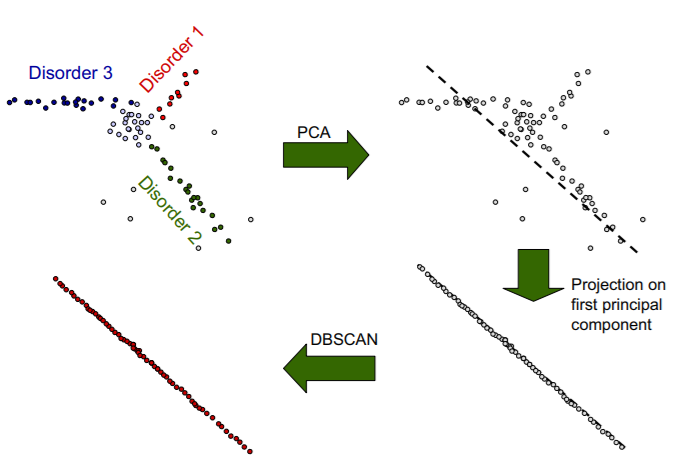
\includegraphics[width=.9\textwidth]{figures/pcalocalfeat1.png}
      \captionof*{figure}{a) First}
      \label{fig:test1}
    \end{minipage}%
    \begin{minipage}[t]{.5\textwidth}
      \centering
      \captionsetup{width=.9\linewidth}
      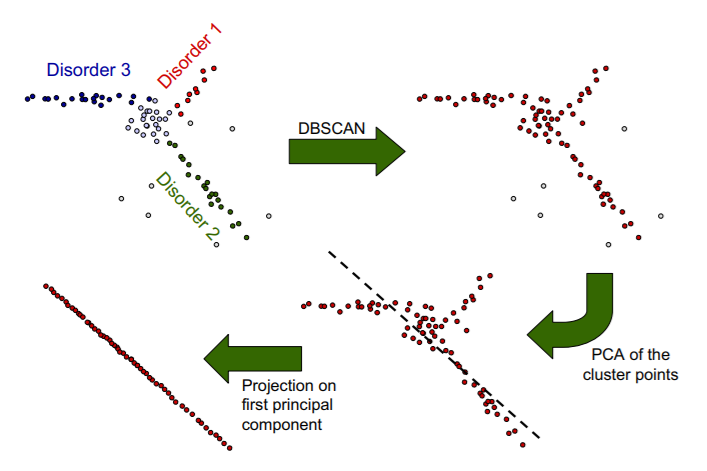
\includegraphics[width=.9\textwidth]{figures/pcalocalfeat2.png}
      \captionof*{figure}{b) Second}
      \label{fig:test2}
    \end{minipage}
    \caption{lazy}
\end{figure}

\subsection{ORCLUS}

\subsection{4C and COPAC}

\subsection{HiCO and ERiC}
(Global) Correlation Clustering, other algorithms so far (ORCLUS \cite{orclusaggarwal2000finding}, LMCLUS \cite{}, 4C, HiCO, ERiC)[1]

Since many of the existing correlation clustering algorithms rely on \gls{pca} they also come with its limitations.

\section{Hough Transformation}\label{sec:houghintro}
The Hough Transform originally was introduced by \textcite{houghOriginal1962method} and extended by \textcite{rosenfeld1969picture} in the field of computer vision for edge detection\cite{houghhistoryhart2009hough}. The initial purpose of the Hough transform was a technique to detect colinear points in an image space but has since then found various other applications in fields like image processing/analysis~\cite{rosenfeld1969picture,ballard1981generalizing}, computer vision~\cite{davies2004machine} and subspace clustering\cite{CASHachtert2008robust}.

The basic idea of the Hough transform is the transformation of all points $p_i = (x_i,y_i)$ in a 2-dimensional image space $\mathcal{D} \subseteq \R^2$ to functions $f_{p_i}$ in a 2-dimensional parameter space $\mathcal{P} \subseteq \R^2$, also known as Hough space\cite{illingworth1988survey}. This is can be done by e.g. taking a representation of a point $p$ as all of its concurrent lines $y_p = m \cdot x_p + t$ and rearranging it to $m_{p} = - \frac{1}{x_p} \cdot t_{p} + \frac{y_p}{x_p}$ which produces a straight with slope $m$ and y-intersect $t$ in a $(m,t)$-parameter space. Since each point in parameter space represents a particular $(m,t)$-setting, multiple functions close to each other implies that their respective points have similar $(m,t)$-settings as well. The correlation clustering objective therefore transforms to a density-based clustering objective in parameter space, with the added benefit of being able to detect correlating points regardless of their distance to each other in data space. This property is exploited by e.g. evaluating the whole parameter space in a grid with a voting scheme or by smartly splitting the parameter space in \autoref{sec:houghintro} to detect linear correlations. 
\todor{Ich plagiere mich selbst. 1zu1 aus unterem abschnitt}
% \begin{figure}
%     \centering
%     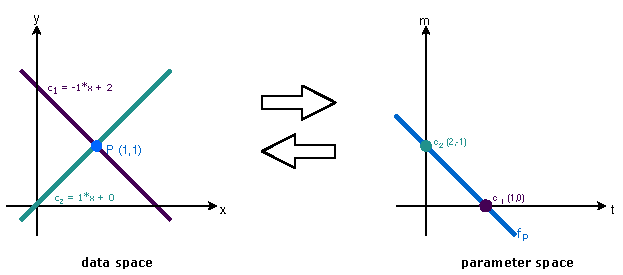
\includegraphics{figures/HoughMXT.pdf}
%     \caption{Caption}
%     \label{fig:houghmxt}
% \end{figure}\todor{eher keine bilder in related work}

\section{CASH}\label{sec:cashintro}
The global correlation clustering algorithm \gls{cash} extends the use case of the Hough Transformation to the detection of arbitrary-dimensional subspaces by augmenting the initial rigid 2-dimensional definition to a multi-dimensional one. 

Furthermore \gls{cash} introduces a improved search strategy for detecting regions of high intersections in parameter space to improve the efficiency compared to the basic grid search \cite{CASHachtert2008global}. Instead of doing an extensive count operation/accumulation of intersections over a fixed interval, \gls{cash} successively splits the whole parameter space by its axes and only further evaluates the split hypercuboids if they contain enough intersections. This is repeated until a certain count of splits is reached and only then hypercuboids with enough intersections are considered as linear correlations. 

Since our work focuses on ``\textit{Detecting Global Correlated Clusters using Hough Transform through Locally Dense Correlations}'', we use \gls{cash} to cope with multi-dimensional data and detect our locally dense correlations. Additionally we will use \gls{cash} as a performance baseline for our descendant algorithm to compare them in a global setting.
A more profound explanation to the transformation and its usage in \gls{cash} will be given in \autoref{ssec:houghindepth}.


\section{DBSCAN}\label{sec:dbscanintro}
\citeauthor{DBSCANEKSX96} created a foundational algorithm with \gls{dbscan}. With over 16000 citations on google scholar as of December 2019 it is one of the most influential works created in the field of density-based clustering and a basis to many clustering approaches, not only restricted to density-based clustering. 

As its name reveals it is an algorithm which detects points in dense vicinity and groups them together. For a measure of density \gls{dbscan} utilizes two parameters. One to specify the minimum amount of neighboring points in a close vicinity and one to specify the range/radius of that vicinity. Points fullfilling these conditions are called \textit{core points} and represent the dense \textit{core} of a cluster. The border of a dense cluster is composed of \textit{border points}. They are points which themselves do not possess a dense neighborhood but are still in the vicinity of core points. 

In contrast to $k$-means-like partitioning clustering\cite{kmeansmacqueen1967some}, \gls{dbscan} is able to find not only non-convex shapes, but also any arbitrary shape of a particular density. Since these arbitrary shaped clusters preserves their correlations and our goal is the assembly of locally dense correlations to global correlations, we expect to obtain good results by partitioning our data space via a density-based algorithm.

\section{OPTICS}\label{sec:OPTICSintro}
A disadvantage of \gls{dbscan} is its dependence on a fixed global parameter setting defining the \textit{minimal} detectable density. Assuming a global linear correlation to have low fluctuations in variance and different global linear correlations having various other variances\todor{can i assume this? i have to do some assumptions right?}, finding clusters with single densities would be more advantageous to our algorithm. We therefore adopted the use of \gls{optics} instead, an improvement/extension of \gls{dbscan}, which enables us to extract single densities more accurately \cite{opticsankerst1999optics}. Since \gls{dbscan} and \gls{optics} are the foundations of the partitioning step we will give a more comprehensive explanations to those two algorithms as well (c.f. \autoref{ssec:DBSCANindepth} and \autoref{ssec:OPTICSindepth}).
% Maybe OPTICS? DIRECTLY COPIED OUT OF \cite{ankerst1999optics}
%  First, almost all clustering algorithms require values for input parameters which are hard to
% determine, especially for real-world data sets containing highdimensional objects. Second, the algorithms are very sensible to
% these parameter values, often producing very different partitionings of the data set even for slightly different parameter settings.
% Third, high-dimensional real-data sets often have a very skewed
% distribution that cannot be revealed by a clustering algorithm using only one global parameter setting. 

% \section{Current Optimization Approaches}
% (D-MASC\cite{kazempour2018d, kazempour2019galaxy}, A Galaxy of Correlations etc.) [0.5] \todor{DMASC ist eigtl nur related work zu CASH aber relevant fuer uns?}
    
